%
% mathFormulierung.tex -- Felder und deren Operationen
%
% 
%
% !TEX root = ../../buch.tex
% !TEX encoding = UTF-8
%
\section{Felder\label{maxwell:mathFormulierung}}
\rhead{Felder}

Da sowohl das elektrische Feld $\vec{E}$ wie auch das magnetische Feld bzw. die magnetische Flussdichte $\vec{B}$ als Vektorfeld beschrieben werden, soll hier der Begriff des Feldes erläutert und grafisch aufgezeigt werden.

\subsection{Skalarfeld\label{maxwell:skalarfeld}}

Ein Skalarfeld ist eine Funktion der Form
\( f:\mathbb{R}^n \rightarrow \mathbb{R}, \) 
die jedem Punkt im Raum ein Skalar zuordnet.
Alltägliches Beispiele für ein Skalarfelder sind Temperaturverteilungen, Ladungsdichten oder Potentiale. In Abbildung \ref{maxwell:skalarGrad} ist ein Skalarfeld abgebildet.


%Zu den wichtigsten Operationen eines Skalarfeldes gehört der Gradient, welcher dem Skalar- ein Vektorfeld zuordnet.
%Sei $\phi$ ein Skalarfeld, dann ist $\nabla\phi$ ein Vektorfeld, dargestellt in \ref{maxwell:skalarGrad}.

\begin{figure}
	\centering
	\subfigure{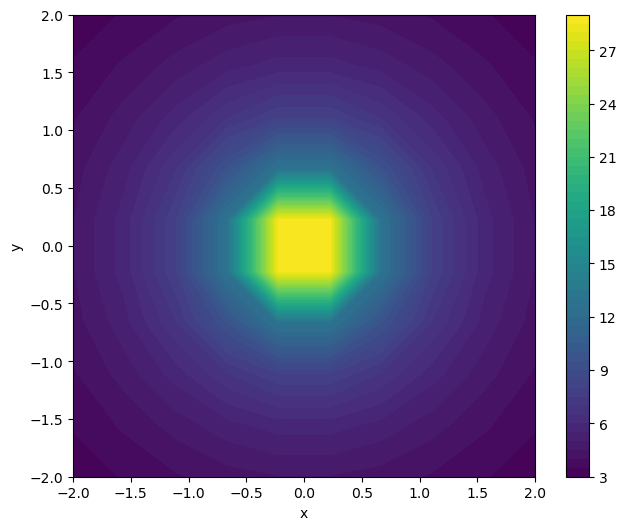
\includegraphics[width=0.35\textwidth]{papers/maxwell/skalar}}
	\subfigure{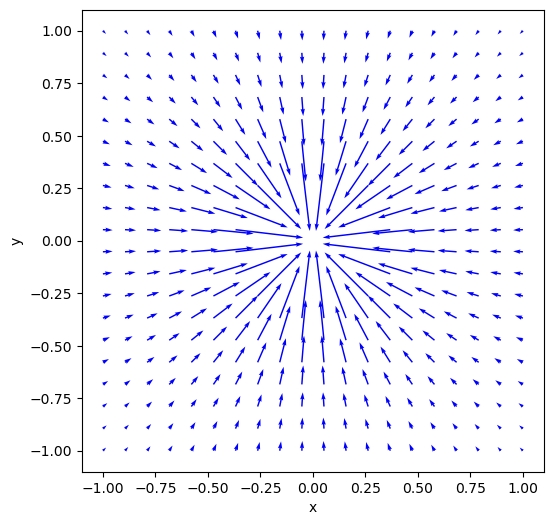
\includegraphics[width=0.3\textwidth]{papers/maxwell/gradient}}
	\caption{Skalar- und Vektorfeld}
	\label{maxwell:skalarGrad}
\end{figure}

\subsection{Vektorfeld\label{maxwell:vektorfeld}}

Ein Vektorfeld ist eine Funktion der Form \( f: \mathbb{R}^n \rightarrow \mathbb{R}^m, \) welche jedem Punkt im Raum einen Vektor zuweist. 
Die Richtung dieses Vektors gibt hierbei an, in welche Richtung der Fluss des Feldes an diesem Punkt geht, während der Betrag die Intensität repräsentiert.


Des weiteren spricht man von einem stationären Vektorfeld, wenn es zeitunabhängig ist und von einem homogenen Vektorfeld, wenn die Richtung und der Betrag der Vektoren ortsunabhängig sind, also wenn jeder Vektor die gleiche Richtung und den gleichen Betrag hat. 
Wie bereits erwähnt, sind das elektrische und das magnetische Feld, wie auch andere Kraftfelder Beispiele von Vektorfeldern.
In Abbildung \ref{maxwell:skalarGrad} ist ein Vektorfeld abgebildet.

\subsection{Operationen}

\subsubsection{Gradient}

Der Gradient einer Funktion $f:\mathbb{R}^3 \rightarrow \mathbb{R}$ ist als 
\[
\renewcommand{\arraystretch}{1.9} 
\operatorname{grad}f = \nabla f = \begin{pmatrix}
\displaystyle
\frac{\partial f}{\partial x} \\
\displaystyle
\frac{\partial f}{\partial y} \\
\displaystyle
\frac{\partial f}{\partial z} \\
\end{pmatrix}\] 
definiert und wurde bereits in Abschnitt \ref{buch:fuvar:richtungsableitung:def:gradient} genauer behandelt. Dieser Operator wird auf ein Skalarfeld angewendet und resultiert in einem Vektorfeld. 
Die Richtung der Vektoren dieses neuen Vektorfeldes zeigen immer in die Richtung der grössten bzw. steilsten Zunahme, wobei der Betrag die Steilheit des Anstiegs repräsentiert.
%Weiter unten wird ersichtlich, dass auch das elektrische Feld ein Gradientenfeld ist \[ \vec{E} = -\nabla\varphi, \] wobei $\varphi$ das elektrische Potential ist.

\subsubsection{Divergenz}
%TODO: Link auf Kapitel von Müller
Die Divergenz eines Vektorfeldes $\vec{F}:\mathbb{R}^3 \rightarrow \mathbb{R}^3$ ist definiert als 
\[ \operatorname{div}\vec{F} = \nabla\cdot\vec{F} 
= \frac{\partial F_x}{\partial x} + \frac{\partial F_y}{\partial y} + \frac{\partial F_z}{\partial z}. \]
Angewendet wird sie auf ein Vektorfeld und resultiert in ein Skalarfeld.
Die Divergenz sagt aus, ob an einem Punkt mehr ``hinein-'' als ``herausfliesst'' und macht so eine Aussage über das Bestehen von Quellen und Senken. 
Wenn die Divergenz negativ ist, liegt eine Senke vor, wenn sie positiv ist eine Quelle.
Ein Vektorfeld wird als quellenfrei bezeichnet, wenn seine Divergenz gleich null ist.

\subsubsection{Rotation}
%TODO: Link auf Kapitel von Müller
Die Rotation eines Vektorfeldes $\vec{F}:\mathbb{R}^3 \rightarrow \mathbb{R}^3$ ist definiert als
\[
\renewcommand{\arraystretch}{1.9} 
\operatorname{rot}\vec{F} = 
\operatorname{curl}\vec{F}
=\nabla\times\vec{F}
= \begin{pmatrix}
	\displaystyle
	\frac{\partial F_z}{\partial y} -\frac{\partial F_y}{\partial z}\\
	\displaystyle
	\frac{\partial F_x}{\partial z} -\frac{\partial F_z}{\partial x}\\
	\displaystyle
	\frac{\partial F_y}{\partial x} -\frac{\partial F_x}{\partial y}
\end{pmatrix}
. \]
Mit dieser Operation wird einem Vektorfeld ein neues Vektorfeld zugeordnet, welches eine Aussage darüber macht, wie stark das Feld sich um einen Punkt dreht bzw. rotiert.
Ein Vektorfeld ist wirbelfrei, wenn seine Rotation null ist.
